\documentclass{article}

\usepackage{booktabs}
\usepackage{graphicx}
\usepackage{caption}
\usepackage{subcaption}

\graphicspath{{../dev/}}

\title{Running Short Initial Analysis}
\author{Ivan Anich}

\begin{document}
\maketitle

This is an initial analysis of a `running short' signal. So far, the results are not great. But, I think that this is because the signal analyzed here is not close to what you have been trading with. The strategy you showed me had a 70\% win rate. I have not been able to recreate such a win rate here, with or without stop losses. Instead I have found the signal to be very noisy: on average returns are not significantly different from zero, and I have had a very hard time finding variants of the signal that are profitable. I have found one such variant, but it is very restrictive: the default signal occurred in over 500 trades across 100 trading days, the variant only occurred in 32. Below I analyze the default signal and this variant, with and without stop losses. I have the stop losses set such that the risk level is either the previous day's high or previous day's close. Moving forward, I can continue to mine this signal for profitable variants. But, we should also talk about how we can make this signal more similar to the strategy it is supposed to represent.

\section{Signal}

The default signal analyzed has three components that all had to be met for the signal to have occurred.

\begin{enumerate}
	\item For each of the three previous days (day -1,-2,-3), the stock closed higher than the previous day's close.
	\item The previous day's high was at least 50\% greater than the open of the fourth previous day (day -4).
	\item The stock gapped down to the current day's (day 0) open.
\end{enumerate}

This is a signal for a short sell. The hypothesis behind it is that the stock is overextended, and so once it gaps down there will be a panic sale, decreasing the price.

I also have analyzed one variation on the default signal signal. It is composed of the first two of components of the default signal, a variation of the third component, and a new component.

\begin{enumerate}
	\item \textit{1 and 2 of the default signal's components.}
	\item The stock is gapping down by magnitude of at least 10\%. 
	\item The open on the current day (day 0) is greater than \$10.
\end{enumerate}

The hypothesis behind the variant is similar to that of the default signal. The larger gap down may increase the panic traders feel if the stock is over extended. The higher open price may mean the stock is overextended to a greater degree, giving it more room to fall.

\section{Results}

Throughout, an entry at the open of day 0 is used. Portfolio simulations are not shown because, for both signals, the percent change in portfolio value was essentially zero. In those simulations, position size was set such that each trade had \$100 of risk. The risk level is set by the difference between the open and either the close or high of the previous day.

\subsection{Default Signal}

Over the 100 trading days prior to May 18th, the default signal occurred 539 times. It is not a strong signal, with or without stop-losses. First, without stop-losses the return of an exit on day 0, either at 10 a.m., 3:30 p.m., or close brings very small negative returns (see figure 1). Holding the stock beyond day 0 leads to worse returns, but not much worse. 

\begin{figure}[!h]
\center{Default Signal: Average Returns}
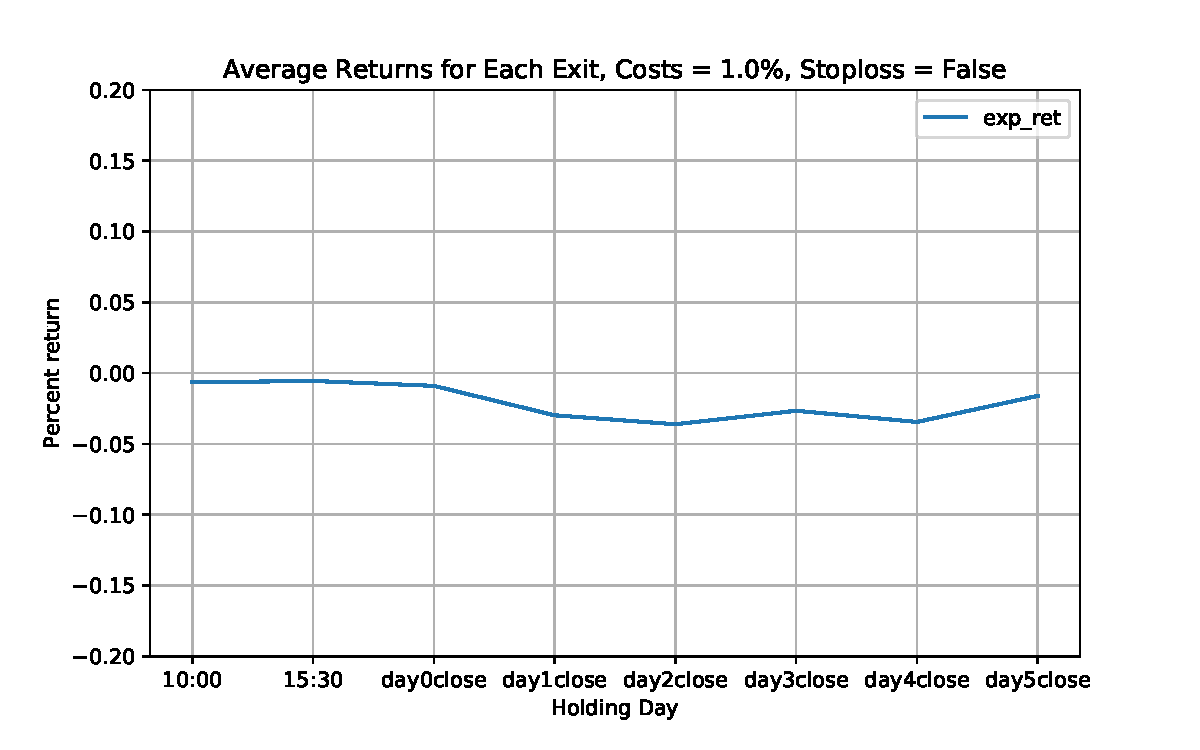
\includegraphics[width=\linewidth]{avg_ret_no_stop_def.pdf}
\caption{The average return for a short trade entered at the open of day 0. The times 10:00 and 15:30 are exits on day 0.}
\end{figure}

With stop losses, the default signal becomes more neutral. The returns to almost all exits are zero regardless of which level risk is set to (see figure 2). Figure 3 shows the percent of trades stopped out of for each exit time analyzed. With the previous day's close as the risk level, about 35\% of trades are stopped out of as of 10 a.m. on day 0. This rises to around 70\% by day 5. With the previous day's high as the risk level, these percentages are much lower, around 10\% and 43\% respectively. The high risk level of the close is less restrictive, but does not substantively change expected returns.

\begin{figure}
\centering
Default Signal: Average Returns w/ Stop-Losses
\begin{subfigure}{\linewidth}
  \centering
  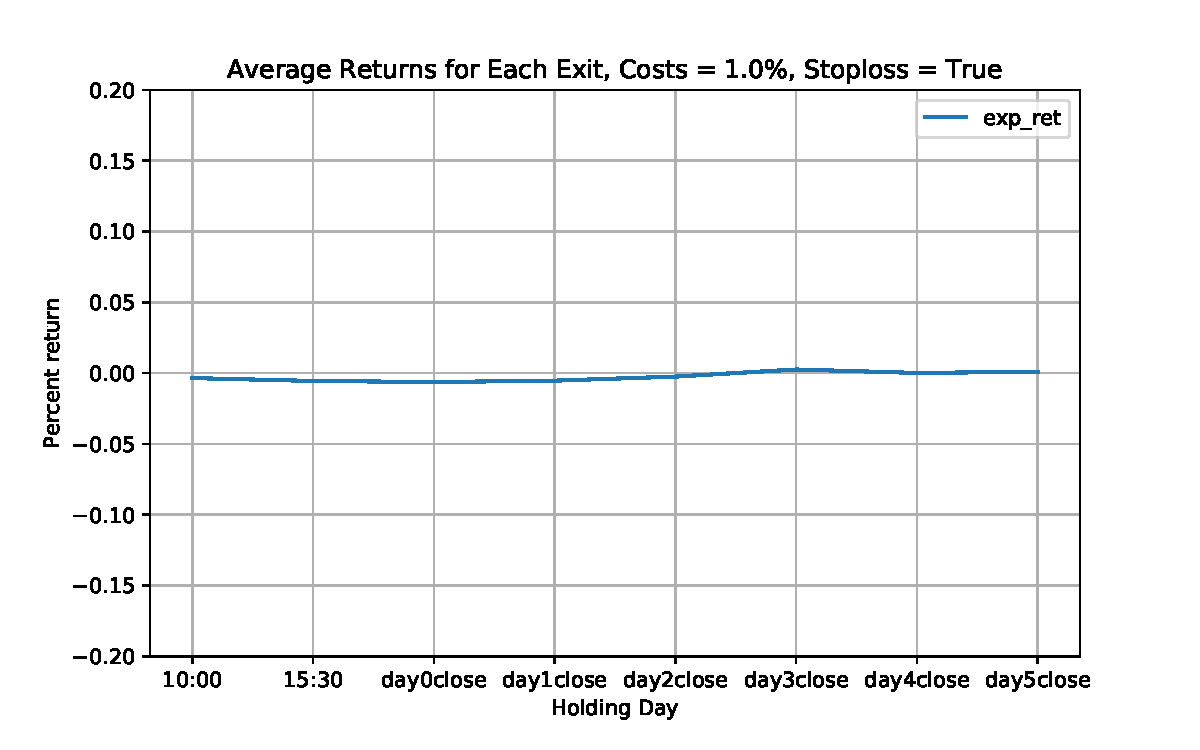
\includegraphics[width=\linewidth]{avg_ret_risk_close.pdf}
  \caption{risk: previous day's close}
\end{subfigure}
\begin{subfigure}{\linewidth}
  \centering
  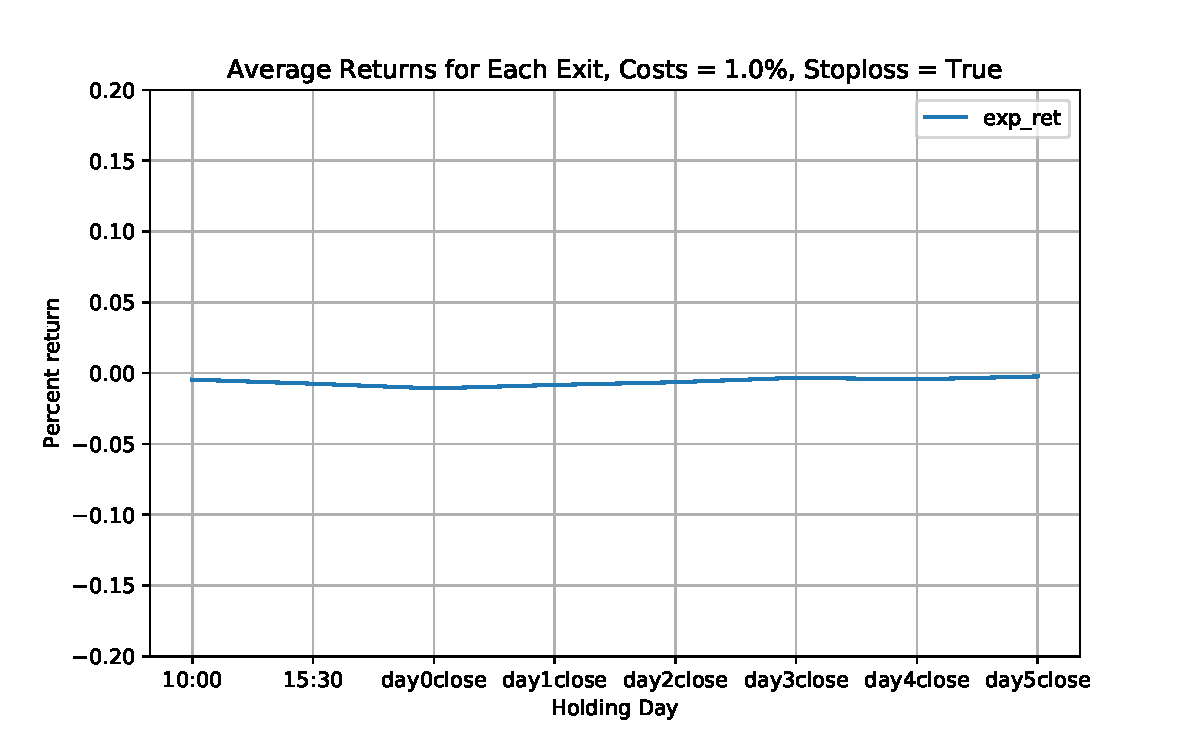
\includegraphics[width=\linewidth]{avg_ret_risk_high.pdf}
  \caption{risk: previous day's high}
\end{subfigure}
\caption{Average returns to default signal with stop losses.}
\end{figure}


\begin{figure}
\centering
Default Signal: Percent of Trades Stopped Out of
\begin{subfigure}{\linewidth}
  \centering
  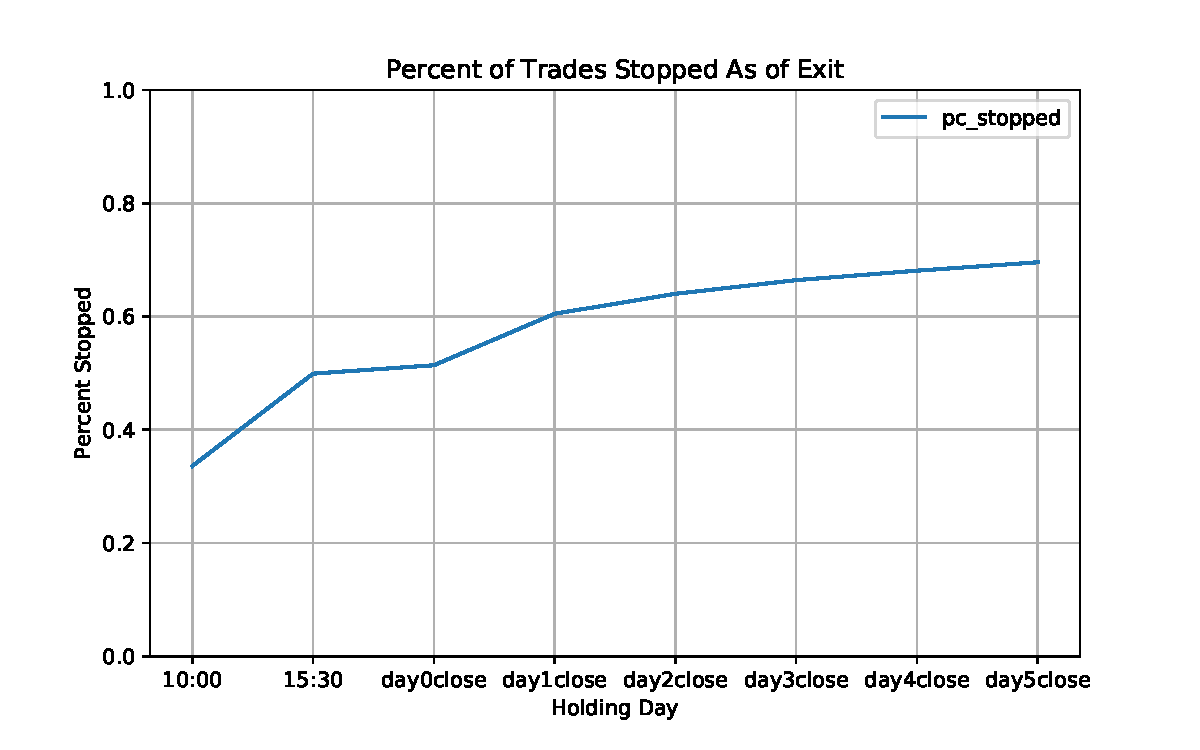
\includegraphics[width=\linewidth]{pc_stop_risk_close.pdf}
  \caption{risk: previous day's close}
\end{subfigure}
\begin{subfigure}{\linewidth}
  \centering
  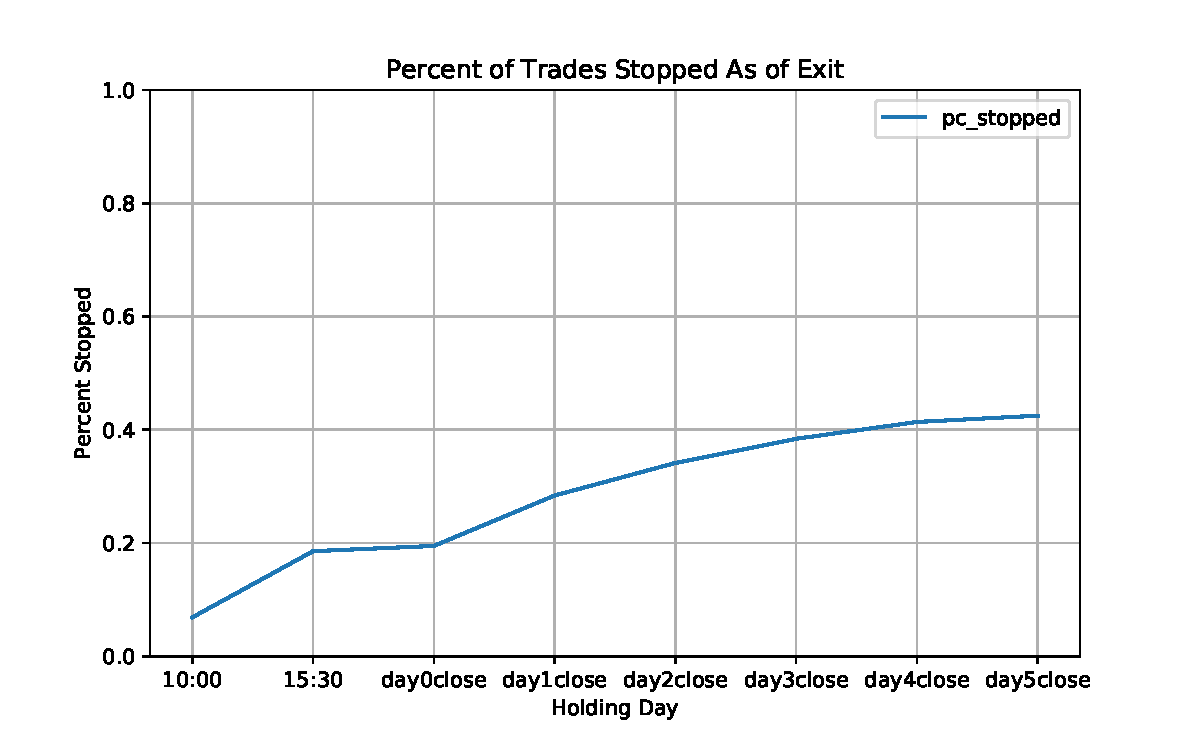
\includegraphics[width=\linewidth]{pc_stop_risk_high.pdf}
  \caption{risk: previous day's high}
\end{subfigure}
\caption{Percent of trades stopped out of, as of each exit time.}
\end{figure}

\subsection{Variant Signal}

Over the 100 trading days prior to May 18th, the variant signal occurred 32 times. It is a stronger signal, but a lot of trades have to be sacrificed in order to limit activity to it and it alone. Figure 4 shows the average returns for each exit without stop losses. There are solid expected returns of just under 5\% for exits at 3:30 pm and at close of day 0. Returns drop when exiting day 1 at close, and then increase until day 5, when an exit at close earns around 16\%.

\begin{figure}[!h]
\center{Variant Signal: Average Returns}
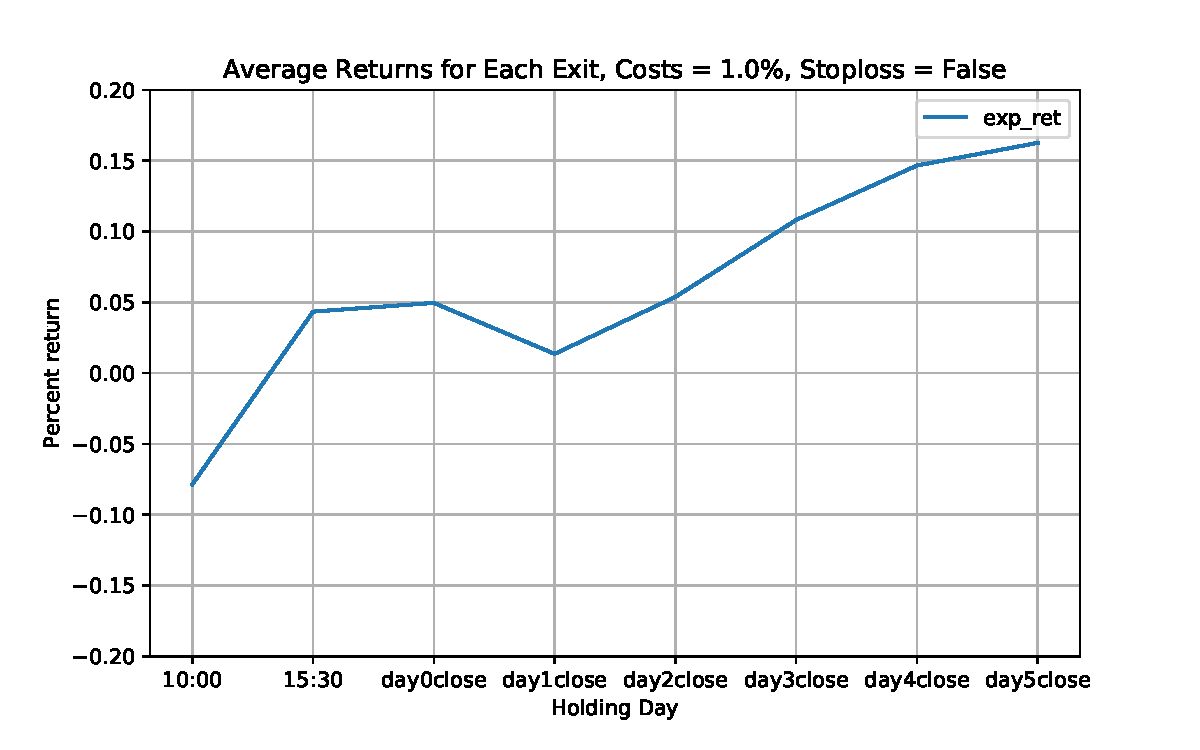
\includegraphics[width=\linewidth]{avg_ret_no_stop_var_1.pdf}
\caption{The average return for a short trade entered at the open of day 0. The times 10:00 and 15:30 are exits on day 0.}
\end{figure}

With stop-losses, the variant signal has lower average returns (see figure 5). Returns for exits at 3:30 pm and close on day 0 are near 2\% for risk levels set at the previous day's high or close. Returns on day 5 are 5\% for a risk level set at the high, and 2.5\% for a risk at the close.

\begin{figure}
\centering
Variant Signal: Average Returns w/ Stop-Losses
\begin{subfigure}{\linewidth}
  \centering
  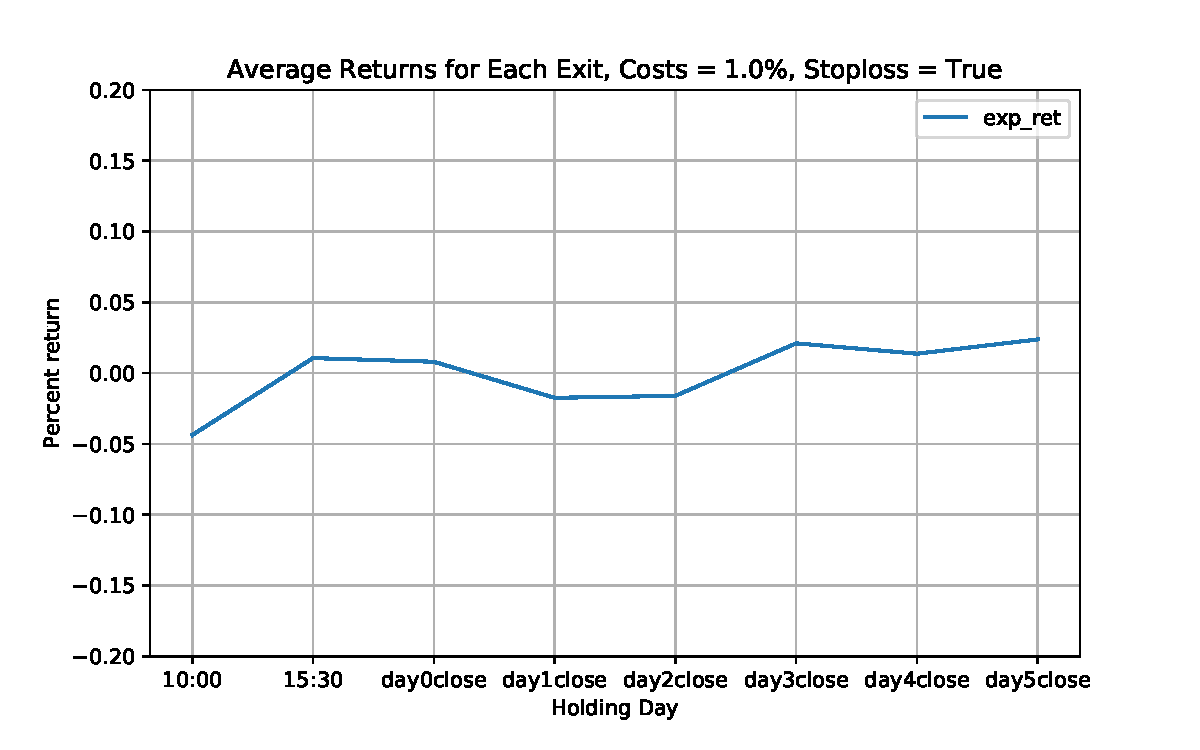
\includegraphics[width=\linewidth]{avg_ret_risk_close_var_1.pdf}
  \caption{risk: previous day's close}
\end{subfigure}
\begin{subfigure}{\linewidth}
  \centering
  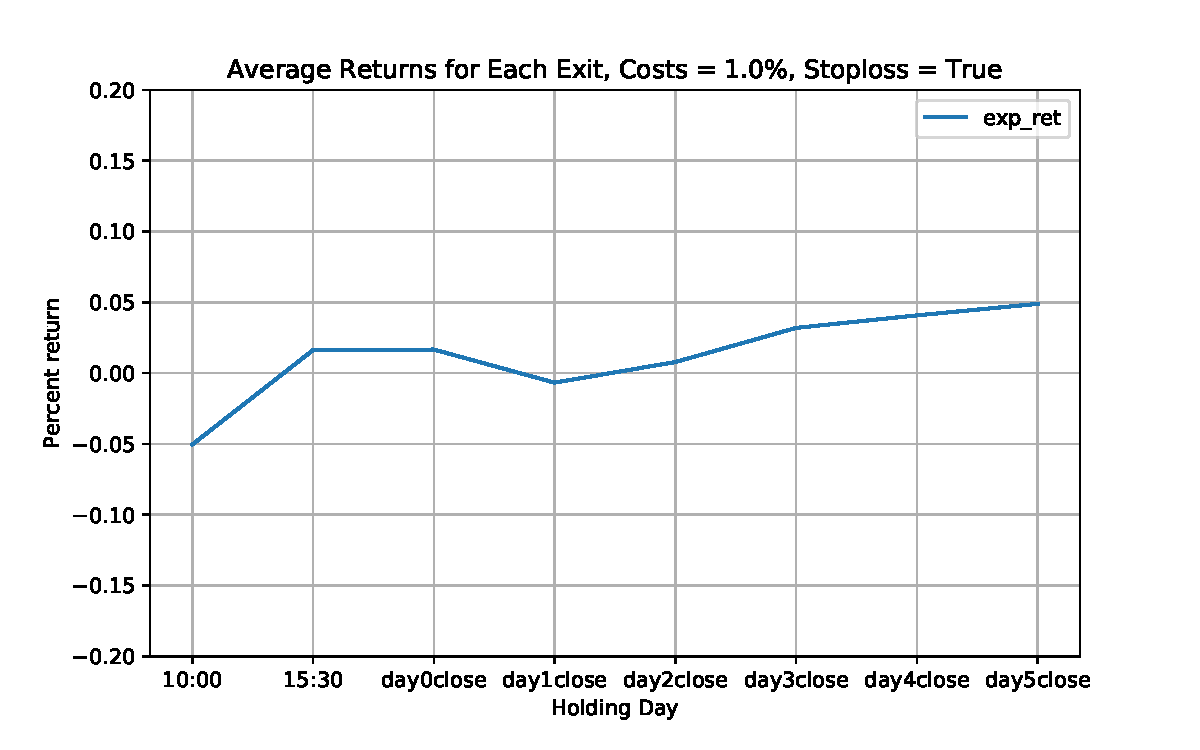
\includegraphics[width=\linewidth]{avg_ret_risk_high_var_1.pdf}
  \caption{risk: previous day's high}
\end{subfigure}
\caption{Average returns to default signal with stop losses.}
\end{figure}


\begin{figure}
\centering
Variant Signal: Percent of Trades Stopped Out Of
\begin{subfigure}{\linewidth}
  \centering
  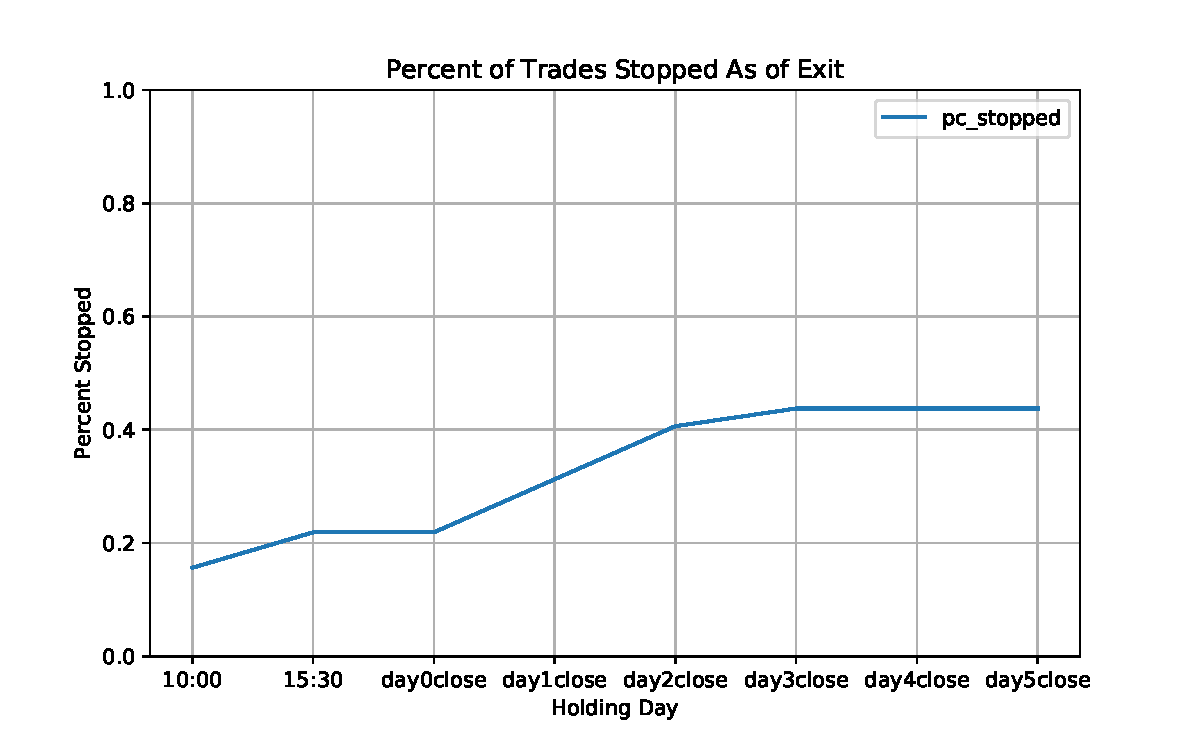
\includegraphics[width=\linewidth]{pc_stop_risk_close_var_1.pdf}
  \caption{risk: previous day's close}
\end{subfigure}
\begin{subfigure}{\linewidth}
  \centering
  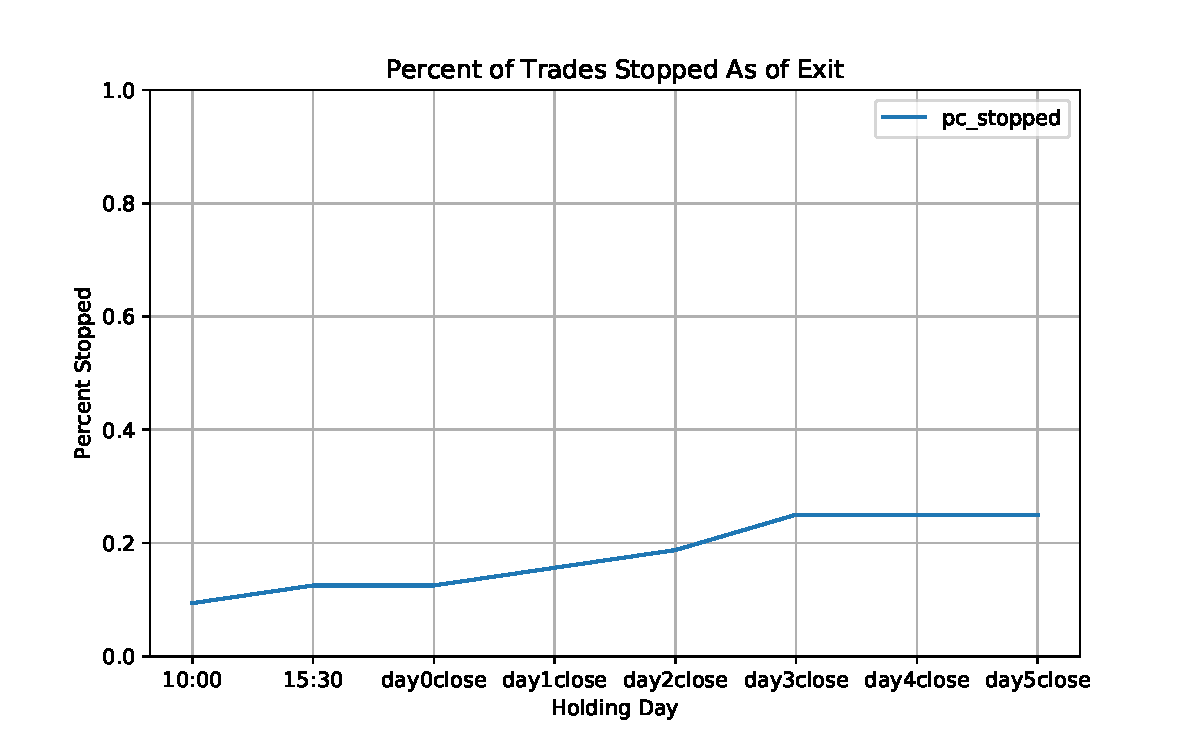
\includegraphics[width=\linewidth]{pc_stop_risk_high_var_1.pdf}
  \caption{risk: previous day's high}
\end{subfigure}
\caption{Percent of trades stopped out of, as of each exit time.}
\end{figure}

Unfortunately, when similating the variant signal, it appears that all of the trades that met the signal had very large risk, so when splitting \$100 of total risk among them, very small position sizes resulted. Gains were very small. The initial portfolio only gained 0.05\%. That being said, if constant position sizes were used, gains would be much higher. 

\section{Conclusion}

Simply put, I don't think the default signal here is exactly what you have been trading with. Your strategy has seen solid returns at a 70\% win rate. No variant of the signal I have tested so far has been able to replicate that. We need to refine the signal such that it more aligns with exactly what you have been trading, then we can start optimizing it more. That being said, there may be some hidden treasure in the default signal that I have yet to find: perhaps with some luck and intuition I can uncover a variant on the signal that is very profitable.

\end{document}